\chapter{Capturas de pantalla}

Este capítulo presenta capturas de pantalla del sistema \textbf{Komuness} implementado, documentando visualmente el progreso alcanzado durante el Sprint 1. 
Las imágenes proporcionan evidencia tangible de las funcionalidades desarrolladas y sirven como registro del estado actual de la plataforma para futuras iteraciones.

Las capturas están organizadas por funcionalidad principal, mostrando tanto la perspectiva del usuario final como las interfaces administrativas. 
Se incluyen vistas en diferentes dispositivos para demostrar la implementación responsive y la adaptabilidad del sistema a diversos contextos de uso.

\section{Capturas del Sistema de Categorías}

Esta sección documenta la implementación completa del sistema de categorías, desde la gestión administrativa hasta la experiencia del usuario final en la clasificación y filtrado de contenido.

\subsection*{Gestión Administrativa de Categorías}

\begin{figure}[H]
  \centering
  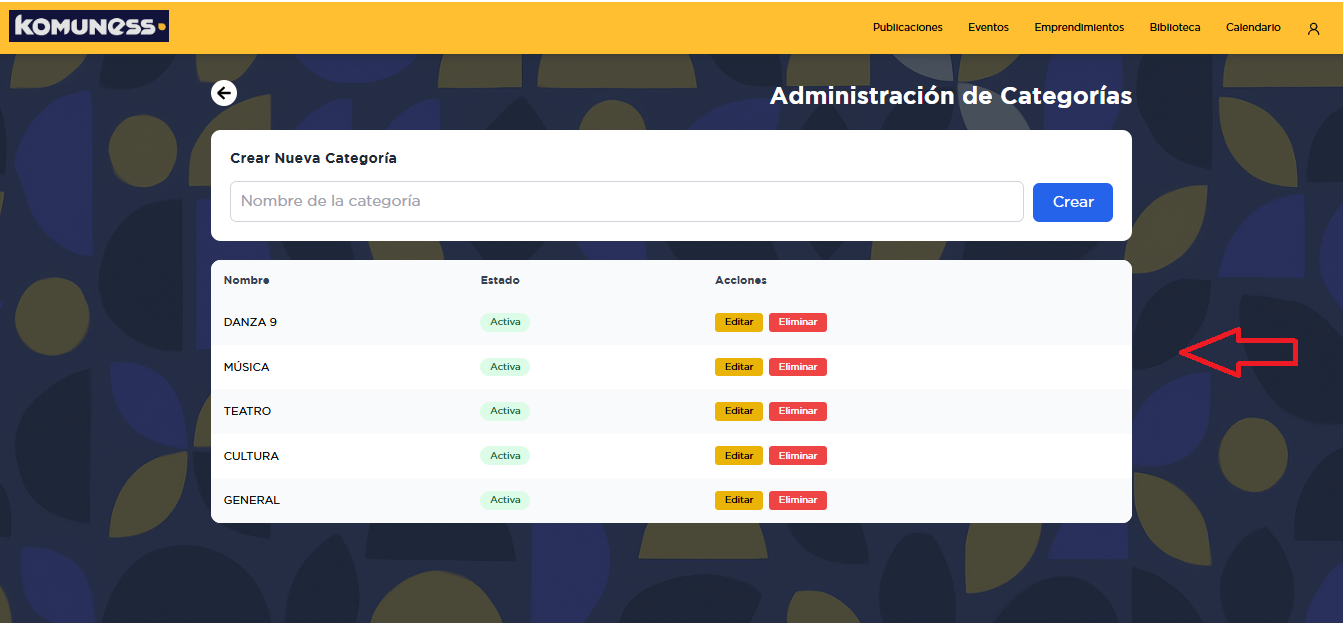
\includegraphics[width=\textwidth]{project/images/6.1.png}
  \caption{Vista principal del panel de administración de categorías mostrando el listado completo con opciones CRUD}
  \label{fig:cat-admin}
\end{figure}

\begin{figure}[H]
  \centering
  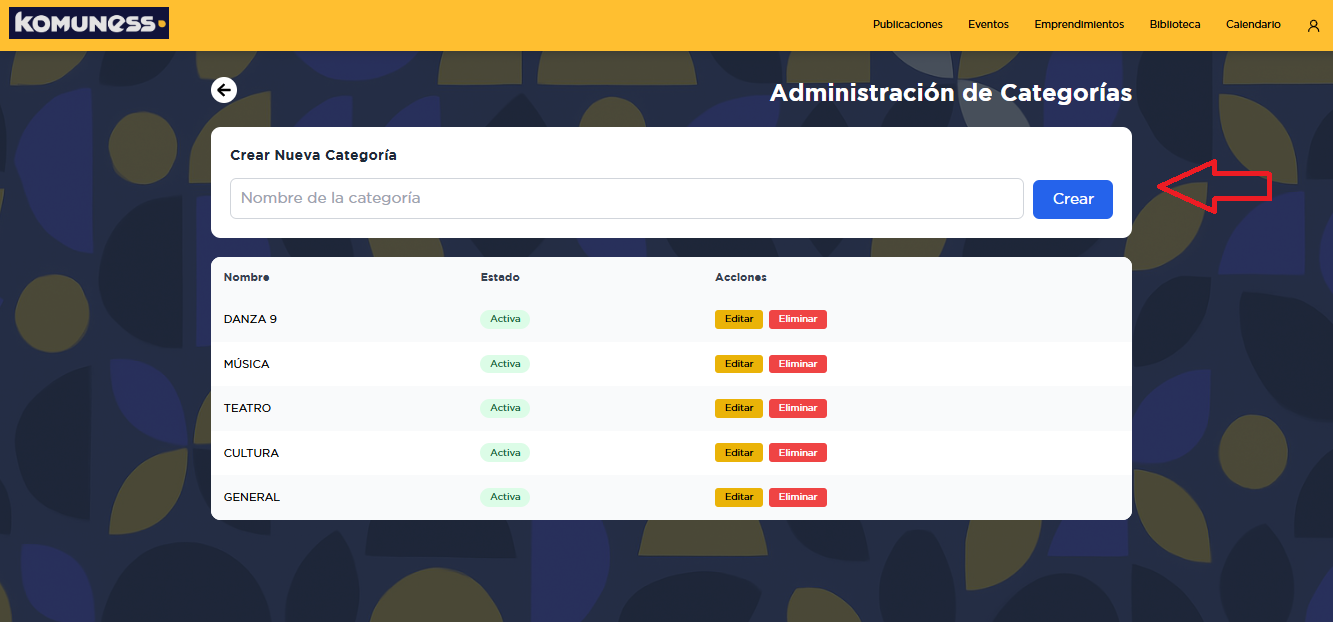
\includegraphics[width=\textwidth]{project/images/6.2.png}
  \caption{Modal de creación de nueva categoría con formulario de validación}
  \label{fig:cat-modal}
\end{figure}

\begin{figure}[H]
  \centering
  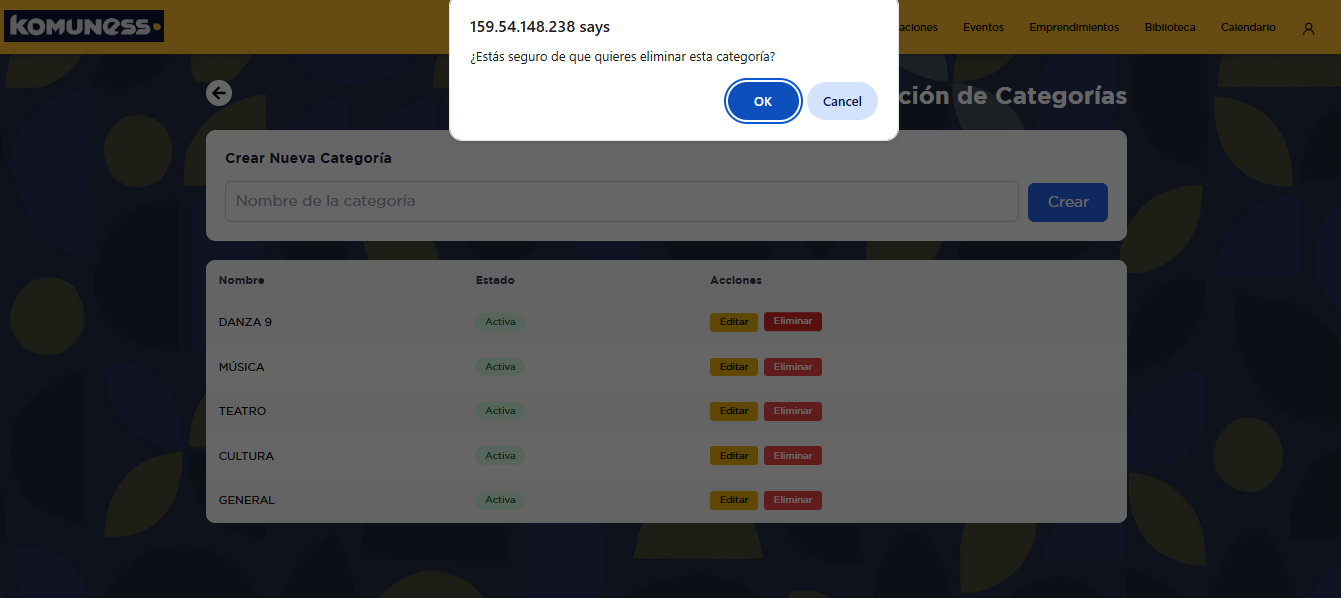
\includegraphics[width=\textwidth]{project/images/6.3.png}
  \caption{Confirmación de eliminación de categoría con advertencia de dependencias}
  \label{fig:cat-delete}
\end{figure}

\subsection*{Experiencia del Usuario con Categorías}

\begin{figure}[H]
  \centering
  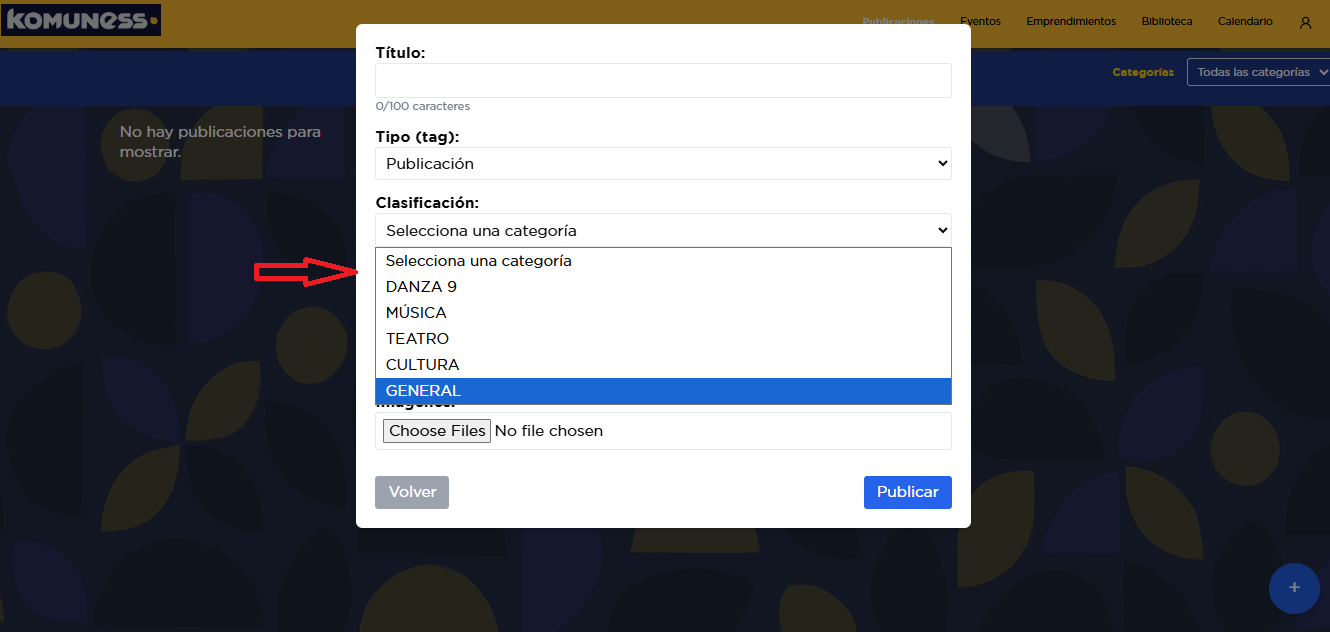
\includegraphics[width=\textwidth]{project/images/6.4.png}
  \caption{Selector de categorías integrado en formulario de creación de publicaciones}
  \label{fig:cat-selector}
\end{figure}


\begin{figure}[H]
  \centering
  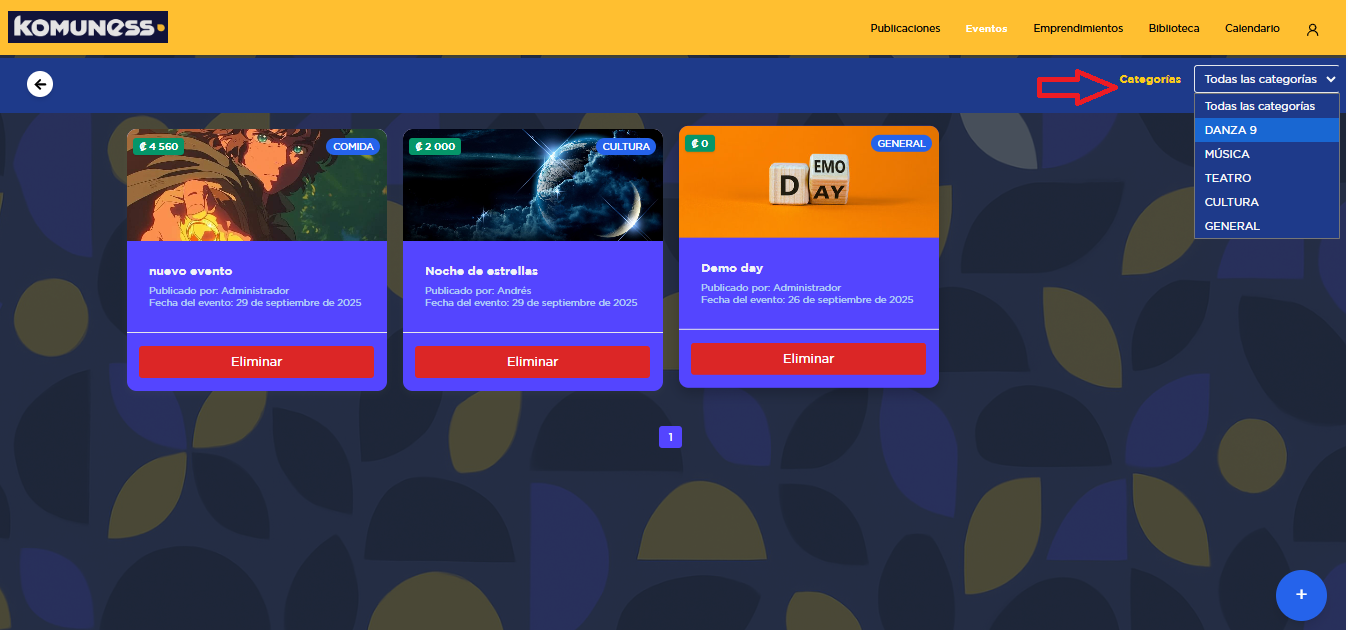
\includegraphics[width=\textwidth]{project/images/6.5.png}
  \caption{Vista de publicaciones filtradas por categoría específica}
  \label{fig:cat-filtradas}
\end{figure}

\section{Capturas del Calendario Interactivo}

\subsection*{Vista Principal del Calendario}

\begin{figure}[H]
  \centering
  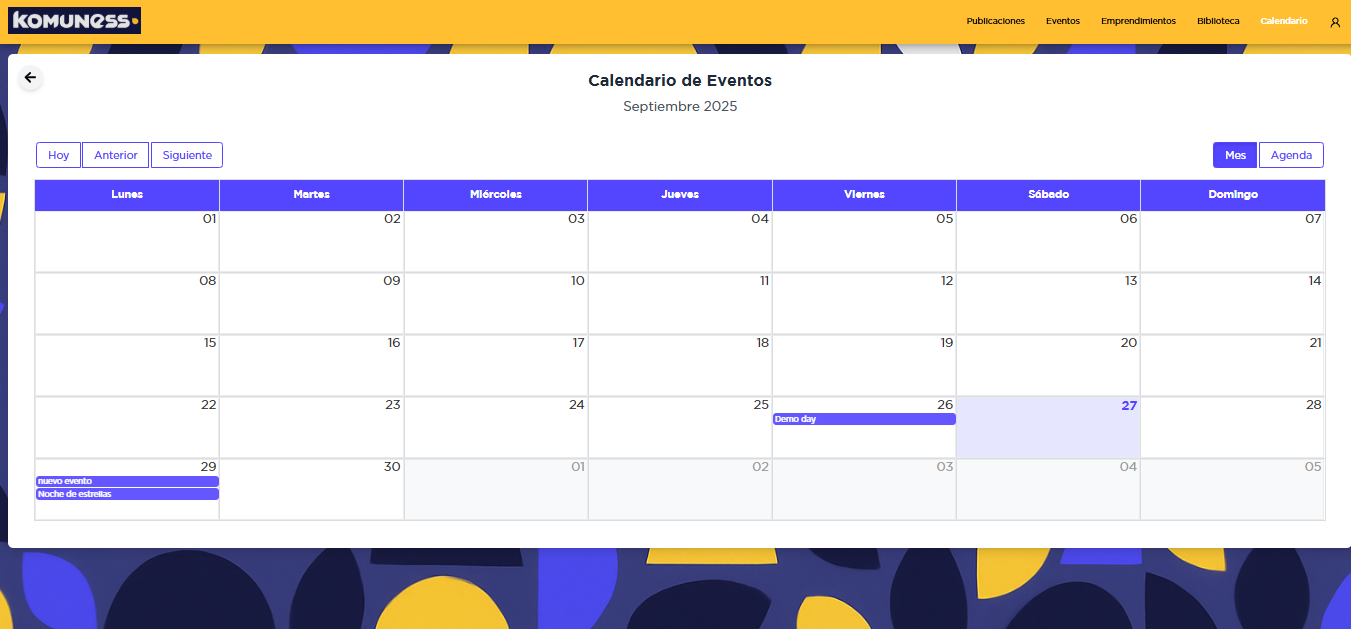
\includegraphics[width=\textwidth]{project/images/6.9.png}
  \caption{Vista mensual del calendario con eventos marcados por fechas}
  \label{fig:cal-mensual}
\end{figure}


\subsection*{Detalles y Gestión de Eventos}

\begin{figure}[H]
  \centering
  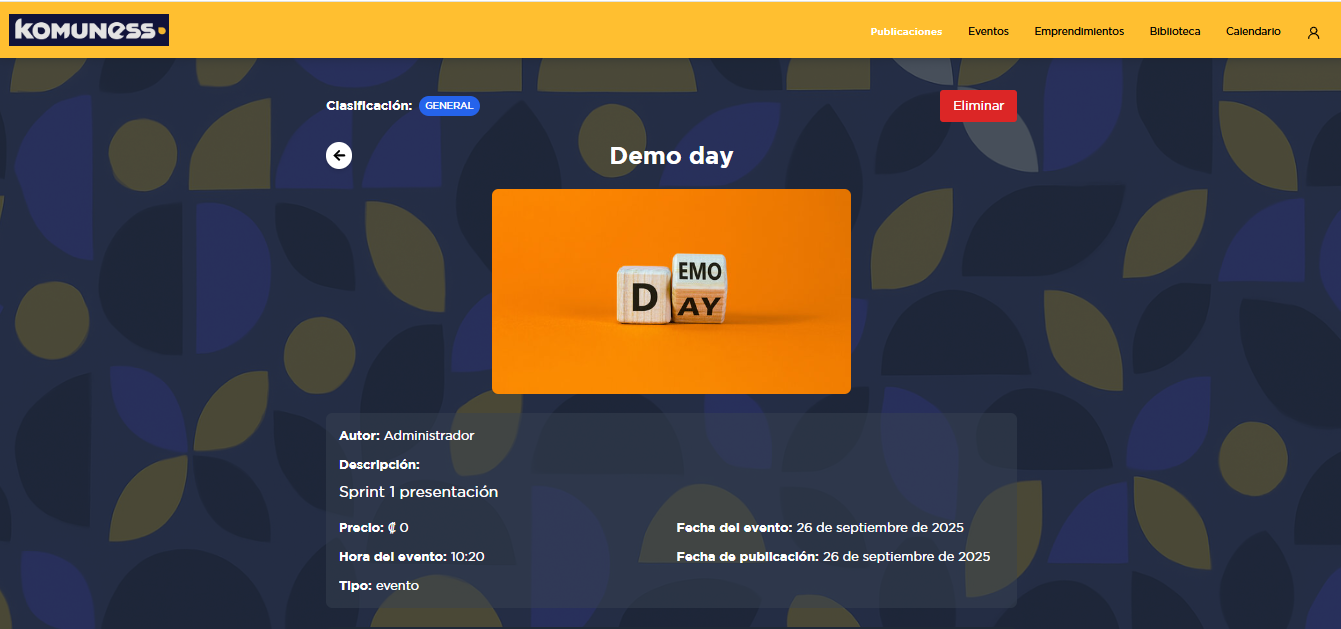
\includegraphics[width=\textwidth]{project/images/6.7.png}
  \caption{Panel de detalles de evento mostrando información completa}
  \label{fig:cal-detalles}
\end{figure}

\begin{figure}[H]
  \centering
  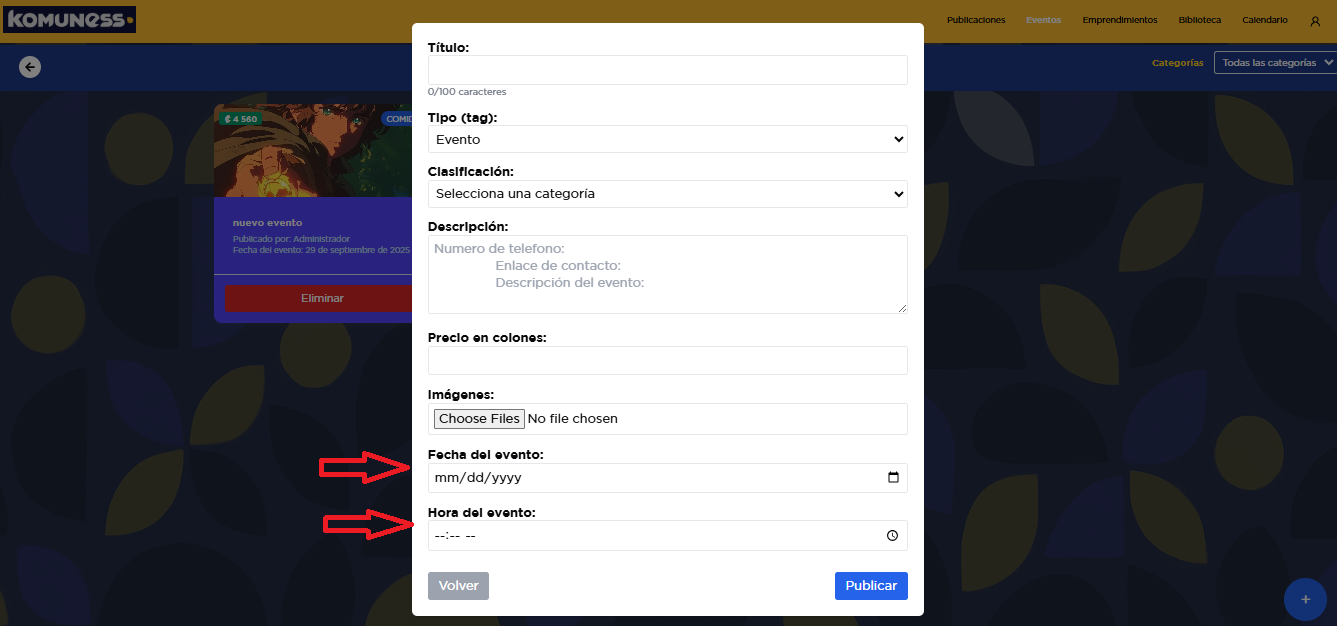
\includegraphics[width=\textwidth]{project/images/6.8.png}
  \caption{Formulario especializado para creación de eventos con campos precio y hora}
  \label{fig:cal-form}
\end{figure}

\begin{figure}[H]
  \centering
  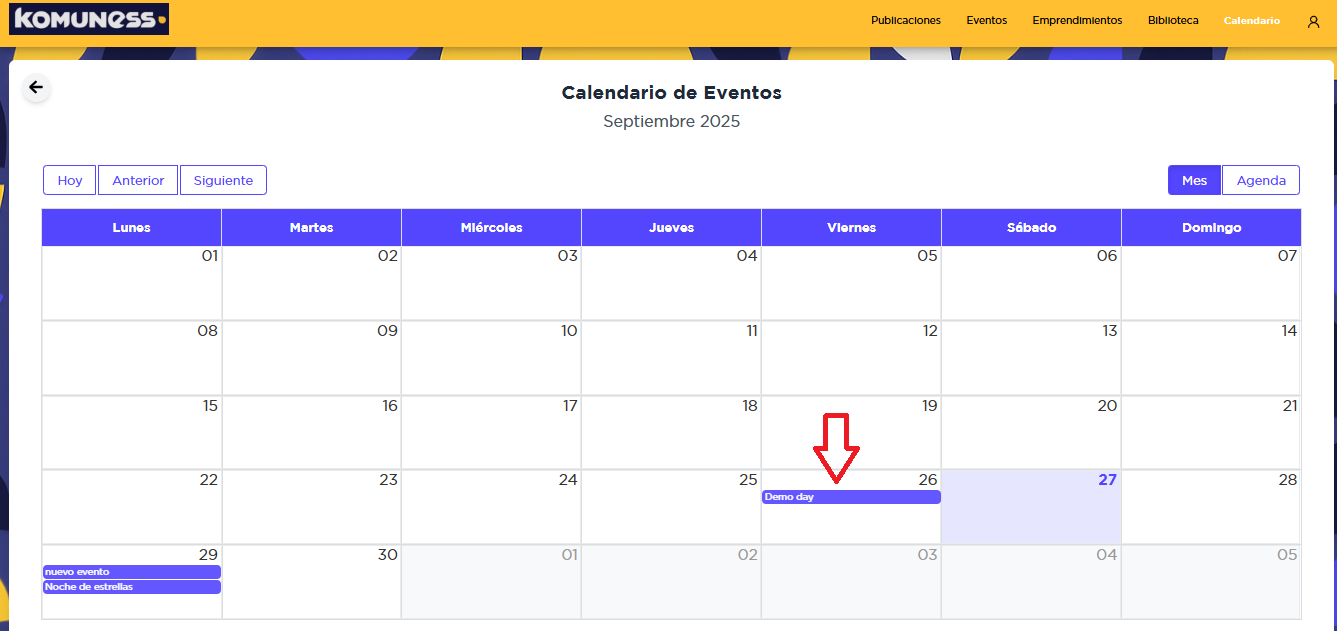
\includegraphics[width=\textwidth]{project/images/6.6}
  \caption{Vista de evento en calendario con dia visible}
  \label{fig:cal-evento}
\end{figure}


\section{Capturas de Mejoras en Biblioteca Digital}

\begin{figure}[H]
  \centering
  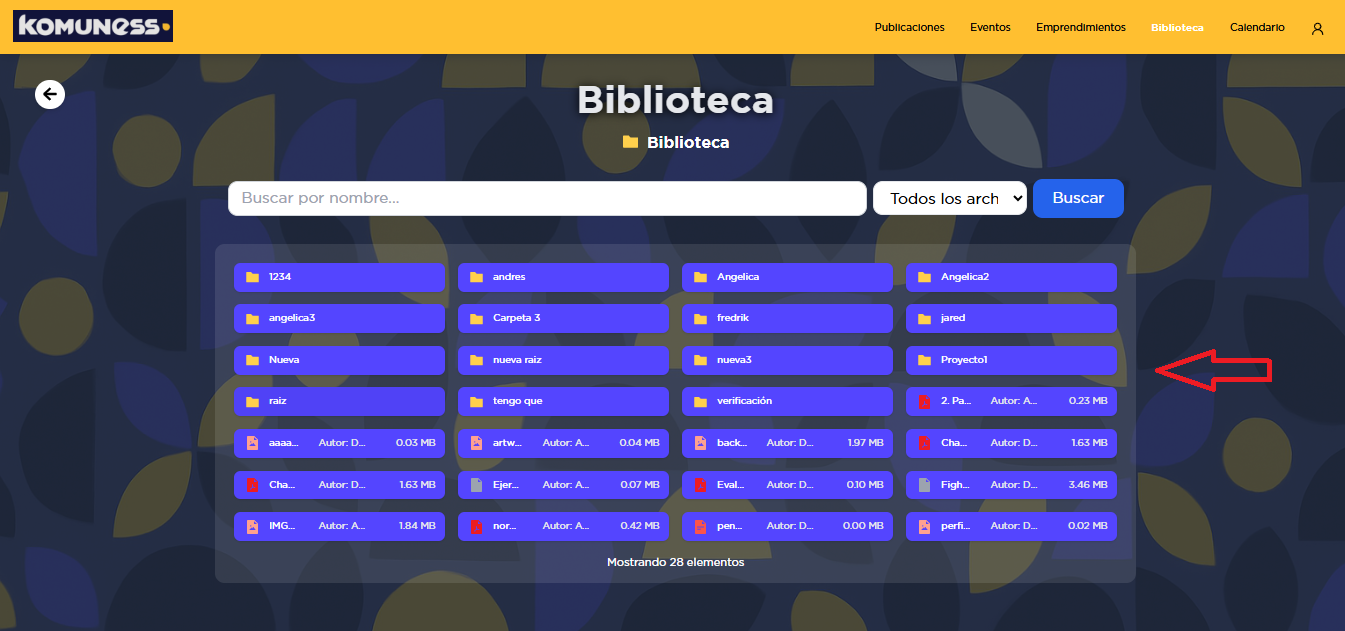
\includegraphics[width=\textwidth]{project/images/6.10.png}
  \caption{Vista optimizada de biblioteca digital con sistema de carpetas mejorado}
  \label{fig:biblio-vista}
\end{figure}


\begin{figure}[H]
  \centering
  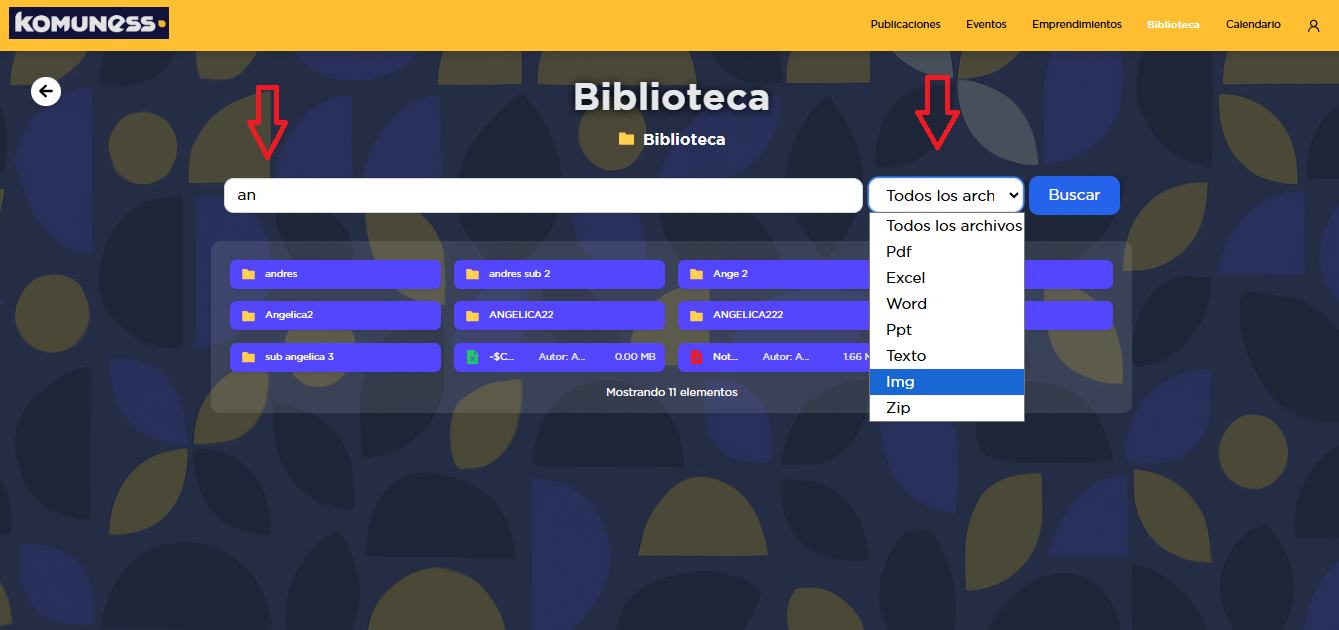
\includegraphics[width=\textwidth]{project/images/6.12}
  \caption{Filtros de búsqueda mejorados en biblioteca digital}
  \label{fig:biblio-filtros}
\end{figure}

\section{Capturas de Adaptación Responsive}

\begin{figure}[H]
  \centering
  % Opción 1: ancho fijo en centímetros
  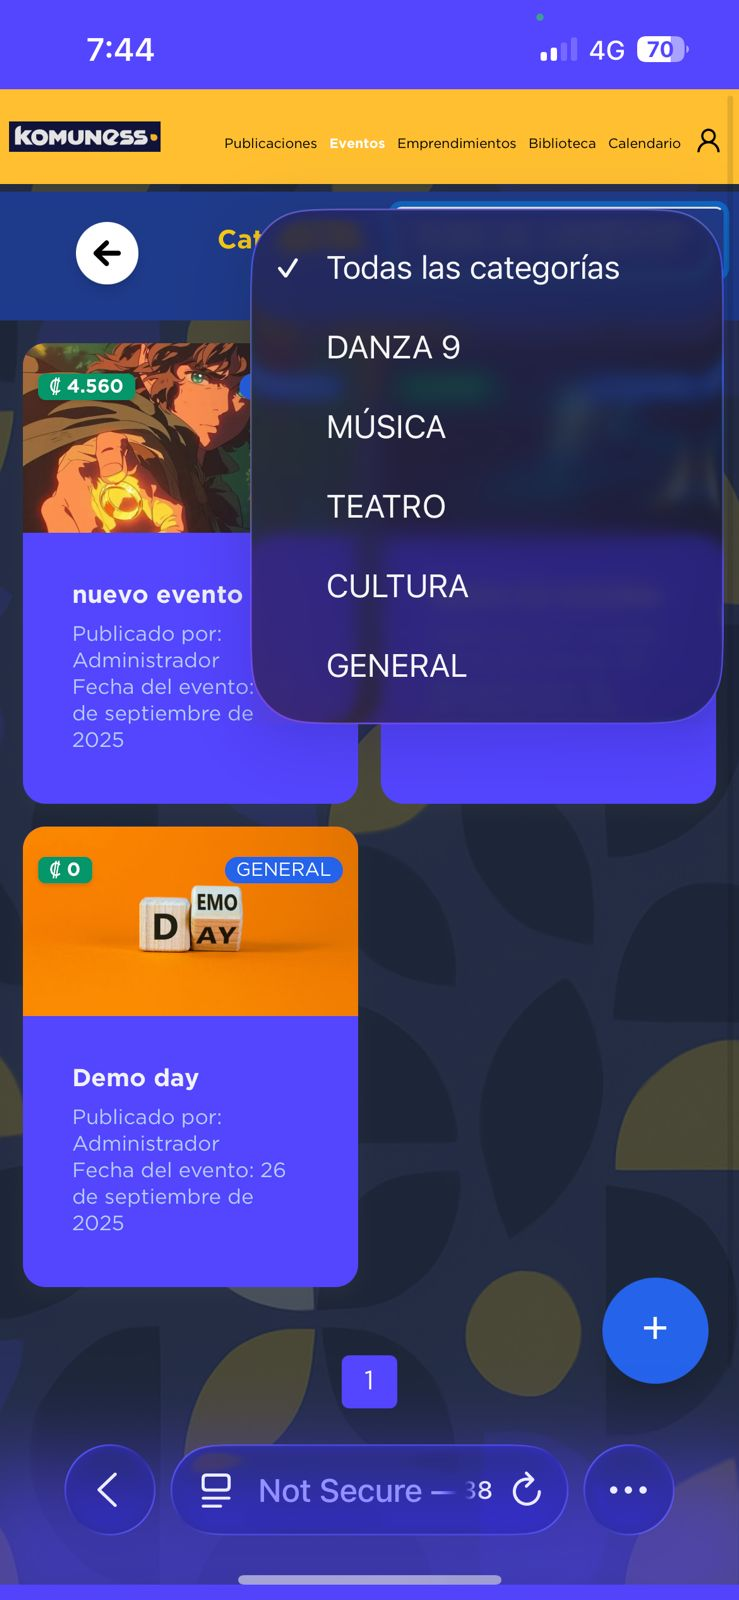
\includegraphics[width=4cm,keepaspectratio]{project/images/imagen13.jpg}
  \caption{Vista móvil del sistema de categorías adaptada para pantallas pequeñas}
  \label{fig:resp-movil}
\end{figure}

\begin{figure}[H]
  \centering
  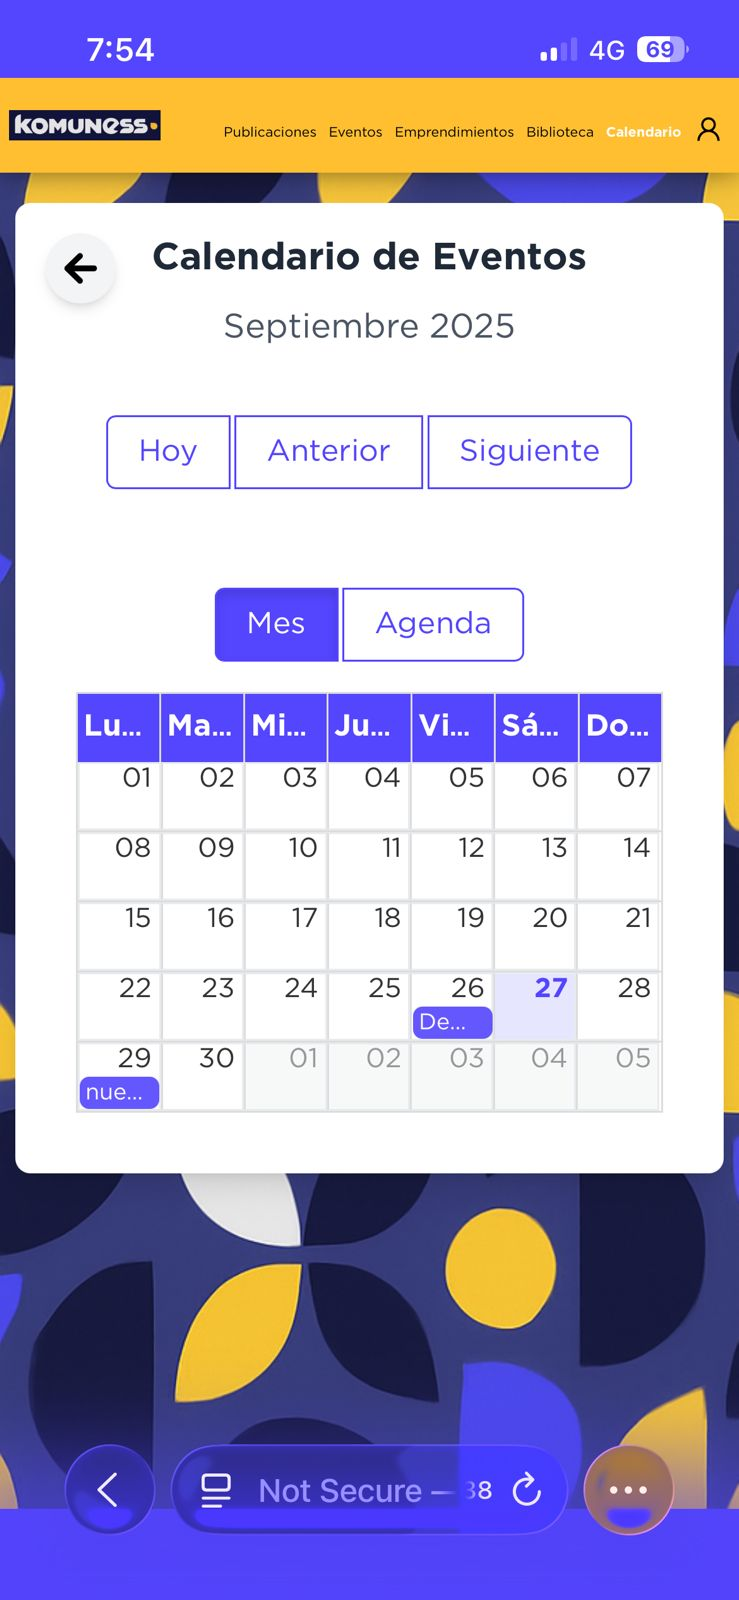
\includegraphics[width=4cm,keepaspectratio]{project/images/imagen14.jpg}
  \caption{Calendario interactivo en dispositivo movil}
  \label{fig:resp-tablet}
\end{figure}

\section{Capturas de Correcciones Frontend}

\begin{figure}[H]
  \centering
  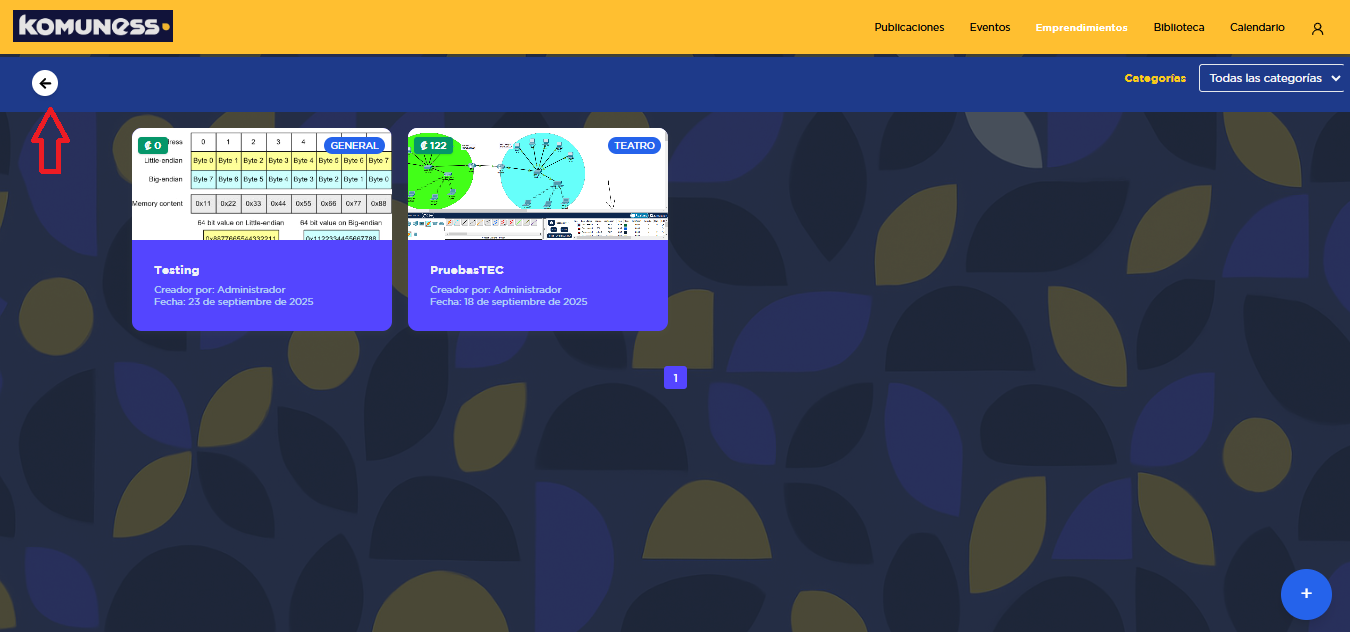
\includegraphics[width=\textwidth]{project/images/6.13.png}
  \caption{Vista de apartados con elementos corregidos y botones ``Volver'' implementados}
  \label{fig:frontend-navegacion}
\end{figure}

\begin{figure}[H]
  \centering
  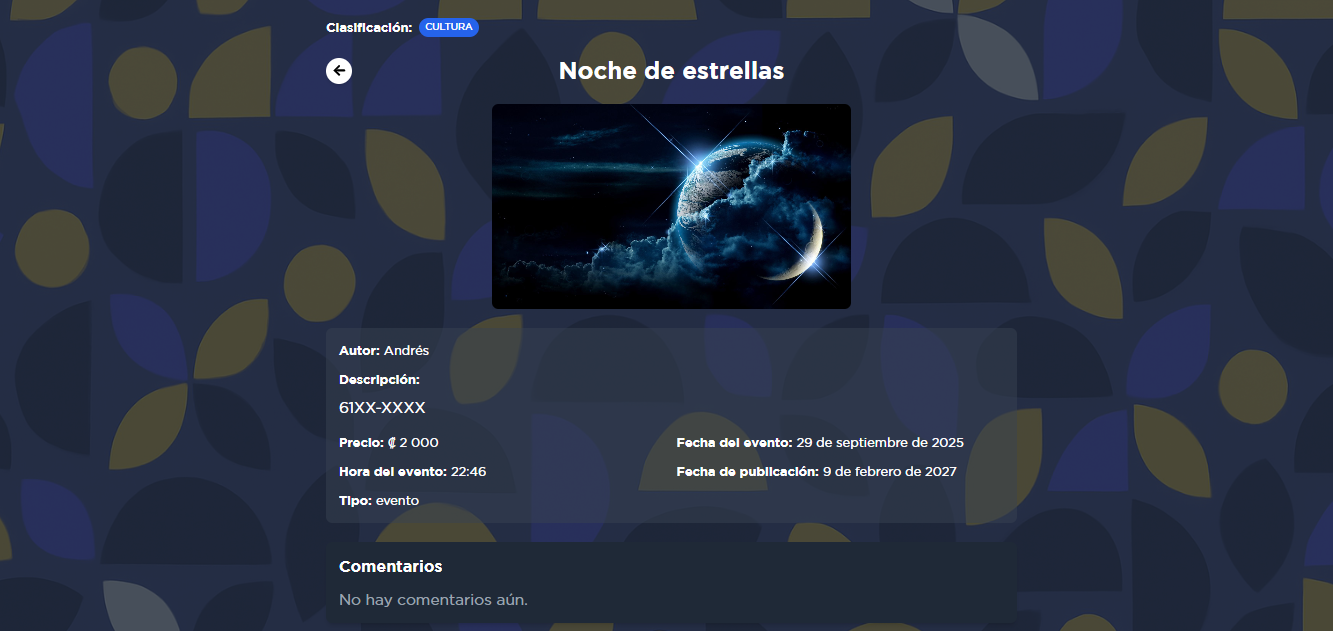
\includegraphics[width=\textwidth]{project/images/6.15.png}
  \caption{Cards de publicaciones con información completa y precio visible}
  \label{fig:frontend-cards}
\end{figure}
